% generated — do not edit
\section{Learned Trigger}\label{sec:trigger}\textcolor{red}{[pending]}

\section{Compact Event Memory}\label{sec:memory}\textcolor{red}{[pending]}

\section{Calibrated Answers and Abstention}\label{sec:calib}\textcolor{red}{[pending]}

\section{Compression and On-Device Port}\label{sec:compress}
\begin{figure}[t]\centering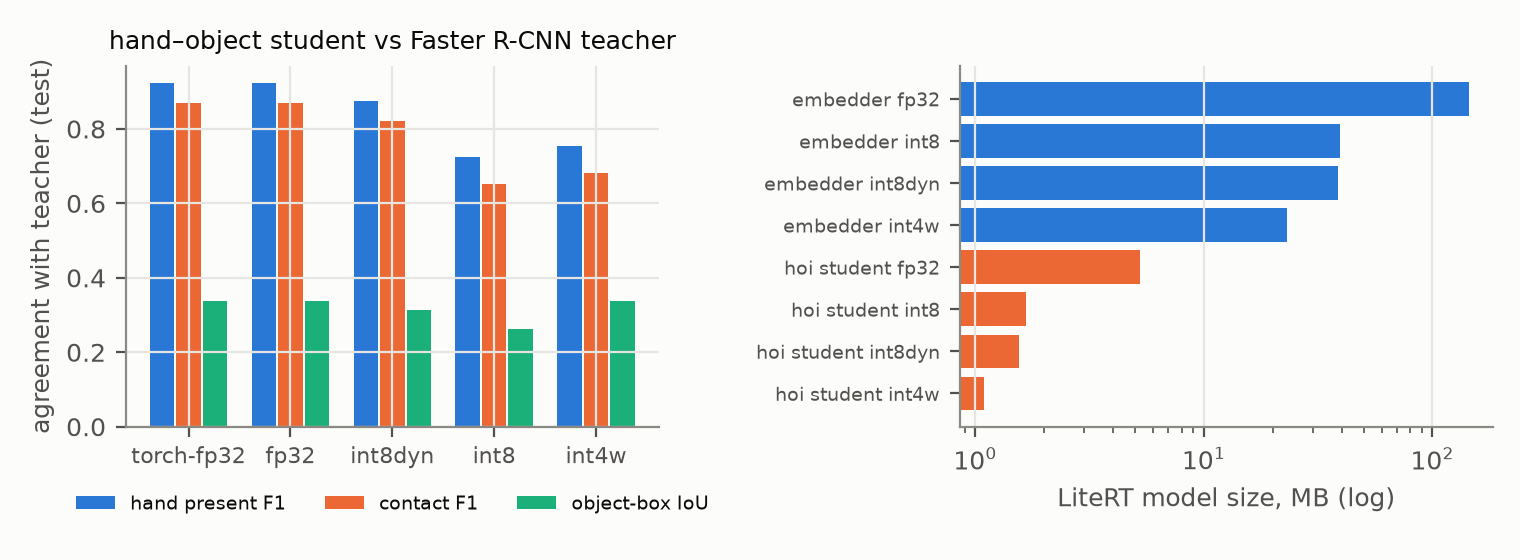
\includegraphics[width=\linewidth]{figs/compression.png}
\caption{Hand--object student agreement with the teacher per precision (left) and LiteRT sizes (right).}\end{figure}
The hand--object student agrees with the Faster R-CNN teacher on held-out frames with hand-present F1 \HoiHandF{} and
contact F1 \HoiContactF{} (\HoiContactFQ{} after dynamic INT8). The embedder goes from \EmbMBfp\,MB to \EmbMBq\,MB with
INT8 weight-only quantisation (cosine to fp32 \EmbCosQ); channel-wise INT4 weights destroy it (cosine \EmbCosFour).
All latency numbers are \emph{desktop-proxy}: no phone was available.

\section{Privacy Layer}\label{sec:privacy}
\begin{figure}[t]\centering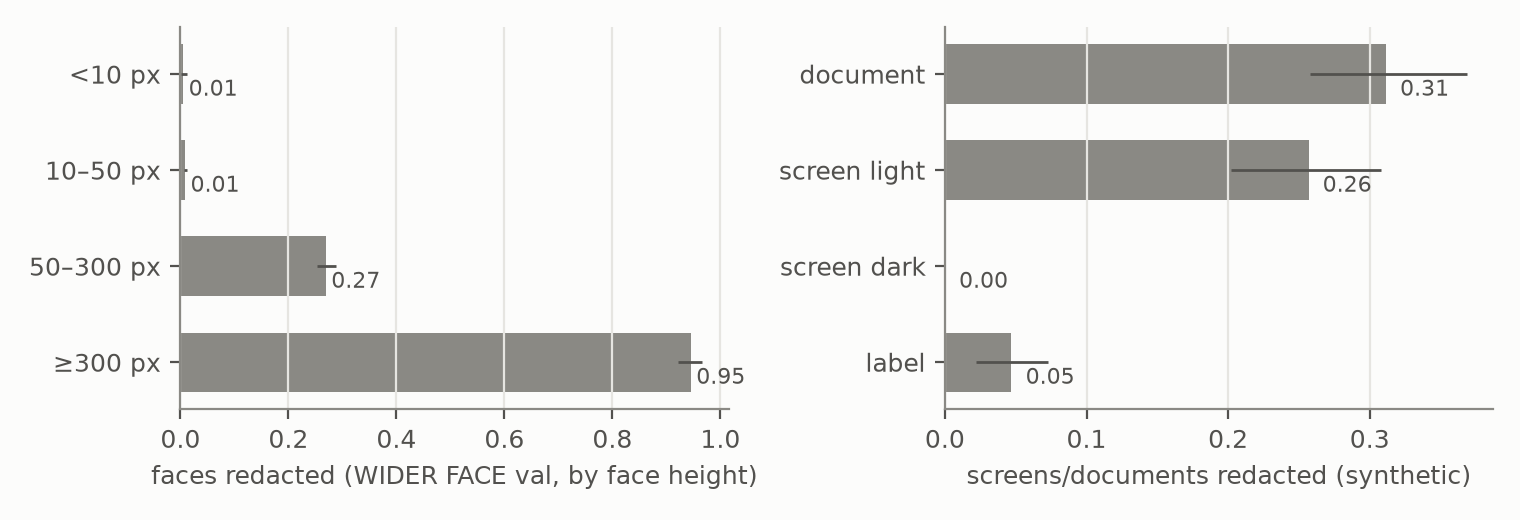
\includegraphics[width=\linewidth]{figs/redaction.png}
\caption{Redaction recall: faces by size (WIDER FACE val) and synthetic screens/documents.}\end{figure}
The redactor catches \FaceLarge{} of faces taller than 300\,px but only \FaceAll{} of all WIDER FACE faces, and
\ScreenAll{} of synthetic screens/documents (none in dark mode). Thumbnails are small event crops, which limits
exposure, but this is the weakest component and is reported as such.

\section{Energy (Estimated)}\label{sec:energy}\textcolor{red}{[pending]}
